% Introduction to ggplot2
% Author: Karthik Ram, karthik.ram@gmail.com
% Licence, CC-BY
\documentclass{beamer}\usepackage{graphicx, color}
%% maxwidth is the original width if it is less than linewidth
%% otherwise use linewidth (to make sure the graphics do not exceed the margin)
\makeatletter
\def\maxwidth{ %
  \ifdim\Gin@nat@width>\linewidth
    \linewidth
  \else
    \Gin@nat@width
  \fi
}
\makeatother

\definecolor{fgcolor}{rgb}{0.2, 0.2, 0.2}
\newcommand{\hlnumber}[1]{\textcolor[rgb]{0,0,0}{#1}}%
\newcommand{\hlfunctioncall}[1]{\textcolor[rgb]{0.501960784313725,0,0.329411764705882}{\textbf{#1}}}%
\newcommand{\hlstring}[1]{\textcolor[rgb]{0.6,0.6,1}{#1}}%
\newcommand{\hlkeyword}[1]{\textcolor[rgb]{0,0,0}{\textbf{#1}}}%
\newcommand{\hlargument}[1]{\textcolor[rgb]{0.690196078431373,0.250980392156863,0.0196078431372549}{#1}}%
\newcommand{\hlcomment}[1]{\textcolor[rgb]{0.180392156862745,0.6,0.341176470588235}{#1}}%
\newcommand{\hlroxygencomment}[1]{\textcolor[rgb]{0.43921568627451,0.47843137254902,0.701960784313725}{#1}}%
\newcommand{\hlformalargs}[1]{\textcolor[rgb]{0.690196078431373,0.250980392156863,0.0196078431372549}{#1}}%
\newcommand{\hleqformalargs}[1]{\textcolor[rgb]{0.690196078431373,0.250980392156863,0.0196078431372549}{#1}}%
\newcommand{\hlassignement}[1]{\textcolor[rgb]{0,0,0}{\textbf{#1}}}%
\newcommand{\hlpackage}[1]{\textcolor[rgb]{0.588235294117647,0.709803921568627,0.145098039215686}{#1}}%
\newcommand{\hlslot}[1]{\textit{#1}}%
\newcommand{\hlsymbol}[1]{\textcolor[rgb]{0,0,0}{#1}}%
\newcommand{\hlprompt}[1]{\textcolor[rgb]{0.2,0.2,0.2}{#1}}%

\usepackage{framed}
\makeatletter
\newenvironment{kframe}{%
 \def\at@end@of@kframe{}%
 \ifinner\ifhmode%
  \def\at@end@of@kframe{\end{minipage}}%
  \begin{minipage}{\columnwidth}%
 \fi\fi%
 \def\FrameCommand##1{\hskip\@totalleftmargin \hskip-\fboxsep
 \colorbox{shadecolor}{##1}\hskip-\fboxsep
     % There is no \\@totalrightmargin, so:
     \hskip-\linewidth \hskip-\@totalleftmargin \hskip\columnwidth}%
 \MakeFramed {\advance\hsize-\width
   \@totalleftmargin\z@ \linewidth\hsize
   \@setminipage}}%
 {\par\unskip\endMakeFramed%
 \at@end@of@kframe}
\makeatother

\definecolor{shadecolor}{rgb}{.97, .97, .97}
\definecolor{messagecolor}{rgb}{0, 0, 0}
\definecolor{warningcolor}{rgb}{1, 0, 1}
\definecolor{errorcolor}{rgb}{1, 0, 0}
\newenvironment{knitrout}{}{} % an empty environment to be redefined in TeX

\usepackage{alltt}
\usepackage{listings}
\usepackage{inconsolata}
\setbeamertemplate{frametitle}[default][center]
\usepackage{url}
\setcounter{secnumdepth}{-1}
\usetheme{Amsterdam}
% --------------------------------------------------------------
% Setting up some knitr options



% --------------------------------------------------------------
\IfFileExists{upquote.sty}{\usepackage{upquote}}{}
\begin{document}
\title{Data Visualization with R \& ggplot2}
\author{Karthik Ram}
\maketitle

% --------------------------------------------------------------
\begin{frame}[fragile]
\frametitle{Download this PDF}
\begingroup
    \fontsize{12pt}{12pt}\selectfont
\href{http://github.com/karthikram/ggplot-lecture}{github.com/karthikram/ggplot-lecture}\\
\href{https://speakerdeck.com/karthik/}{https://speakerdeck.com/karthik/}
\endgroup
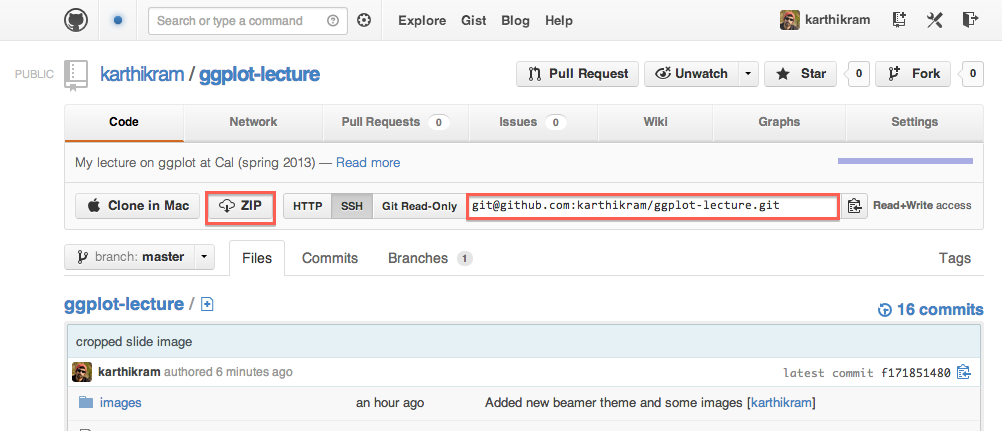
\includegraphics[scale=.31]{images/git_repo.png}
\end{frame}

% --------------------------------------------------------------
\begin{frame}[fragile]
\frametitle{Some housekeeping}
Install some packages
\begin{knitrout}\footnotesize
\definecolor{shadecolor}{rgb}{0.969, 0.969, 0.969}\color{fgcolor}\begin{kframe}
\begin{alltt}
\hlfunctioncall{install.packages}(\hlstring{"ggplot2"}, dependencies = TRUE)
\end{alltt}
\end{kframe}
\end{knitrout}

\end{frame}



% --------------------------------------------------------------
\begin{frame}[fragile]
\frametitle{Base graphics}
\begin{itemize}
\item Ugly, laborious, and verbose\\
\item There are better ways to describe statistical visualizations.\\
\end{itemize}
\end{frame}

\begin{frame}[fragile]
\frametitle{Why \texttt{ggplot2}?}
\begin{itemize}
\item Follows a grammar, just like any language.
\item It defines basic components that make up a sentence. In this case, the grammar defines components in a plot.
\item Grammar of graphics originally coined by Lee Wilkinson
\end{itemize}
\end{frame}


% --------------------------------------------------------------
\begin{frame}[fragile]
\frametitle{Why \texttt{ggplot2}?}
\begin{itemize}
\item  Supports a continuum of expertise.
\item Get started right away but with practice you can effortless build complex, publication quality figures.
\end{itemize}
\end{frame}

% --------------------------------------------------------------
\section*{Basics}
\frame{\sectionpage}


\begin{frame}[fragile]
\frametitle{Some terminology}
\begin{itemize}
\item \textbf{ggplot} - The main function where you specify the dataset and variables to plot\\
\item \textbf{geoms} - geometric objects
    \begin{itemize}
    \item geom\_point(), geom\_bar(), geom\_density(), geom\_line(), geom\_area()
    \end{itemize}
\item \textbf{aes} -  aesthetics
        \begin{itemize}
    \item shape, transparency (alpha), color, fill, linetype.
    \end{itemize}
\item \textbf{scales}  Define how your data will be plotted
        \begin{itemize}
    \item \emph{continuous}, \emph{discrete}, \emph{log}
    \end{itemize}
\end{itemize}
\end{frame}


% --------------------------------------------------------------
\section*{Assembling your first ggplot}
\frame{\sectionpage}

% --------------------------------------------------------------
\begin{frame}[fragile]
\frametitle{The iris dataset}
\begin{knitrout}\footnotesize
\definecolor{shadecolor}{rgb}{0.969, 0.969, 0.969}\color{fgcolor}\begin{kframe}
\begin{alltt}
\hlfunctioncall{head}(iris)
\end{alltt}
\begin{verbatim}
##   Sepal.Length Sepal.Width Petal.Length Petal.Width Species
## 1          5.1         3.5          1.4         0.2  setosa
## 2          4.9         3.0          1.4         0.2  setosa
## 3          4.7         3.2          1.3         0.2  setosa
## 4          4.6         3.1          1.5         0.2  setosa
## 5          5.0         3.6          1.4         0.2  setosa
## 6          5.4         3.9          1.7         0.4  setosa
\end{verbatim}
\end{kframe}
\end{knitrout}

\end{frame}

% --------------------------------------------------------------
\begin{frame}[fragile]
\frametitle{Let's try an example}
\begin{knitrout}\footnotesize
\definecolor{shadecolor}{rgb}{0.969, 0.969, 0.969}\color{fgcolor}\begin{kframe}
\begin{alltt}
\hlfunctioncall{ggplot}(data = iris, \hlfunctioncall{aes}(x = Sepal.Length, y = Sepal.Width)) +
\hlfunctioncall{geom_point}()
\end{alltt}
\end{kframe}
\includegraphics[width=.75\linewidth]{figure/first_plot_} 

\end{knitrout}

\end{frame}

% --------------------------------------------------------------
\begin{frame}[fragile]
\frametitle{Basic structure}
\begin{knitrout}\footnotesize
\definecolor{shadecolor}{rgb}{0.969, 0.969, 0.969}\color{fgcolor}\begin{kframe}
\begin{alltt}
\hlfunctioncall{ggplot}(data = iris, \hlfunctioncall{aes}(x = Sepal.Length, y = Sepal.Width))
 + \hlfunctioncall{geom_point}()
myplot <- \hlfunctioncall{ggplot}(data = iris, \hlfunctioncall{aes}(x = Sepal.Length, y = Sepal.Width))
myplot + \hlfunctioncall{geom_point}()
\end{alltt}
\end{kframe}
\end{knitrout}

\begin{itemize}
\item Specify the data and variables inside the \texttt{ggplot} function.
\item Anything else that goes in here becomes a global setting.
\item Then add layers of geometric objects, statistical models, and panels.
\end{itemize}
\end{frame}

% --------------------------------------------------------------
\begin{frame}[fragile]
\frametitle{Quick note}
\begin{itemize}
\item Never use \texttt{qplot} - short for quick plot.
\item You'll end up unlearning and relearning a good bit.
\end{itemize}

\end{frame}


% --------------------------------------------------------------
\begin{frame}[fragile]
\frametitle{Increase the size of points}
\begin{knitrout}\footnotesize
\definecolor{shadecolor}{rgb}{0.969, 0.969, 0.969}\color{fgcolor}\begin{kframe}
\begin{alltt}
\hlfunctioncall{ggplot}(data = iris, \hlfunctioncall{aes}(x = Sepal.Length, y = Sepal.Width)) +
\hlfunctioncall{geom_point}(size = 3)
\end{alltt}
\end{kframe}
\includegraphics[width=.75\linewidth]{figure/first_plot_size_} 

\end{knitrout}

\end{frame}

% --------------------------------------------------------------
\begin{frame}[fragile]
\frametitle{Add some color}
\begin{knitrout}\footnotesize
\definecolor{shadecolor}{rgb}{0.969, 0.969, 0.969}\color{fgcolor}\begin{kframe}
\begin{alltt}
\hlfunctioncall{ggplot}(iris, \hlfunctioncall{aes}(Sepal.Length, Sepal.Width, color = Species)) +
\hlfunctioncall{geom_point}(size = 3)
\end{alltt}
\end{kframe}
\includegraphics[width=.75\linewidth]{figure/first_plot_color_} 

\end{knitrout}

\end{frame}

% --------------------------------------------------------------
\begin{frame}[fragile]
\frametitle{Differentiate points by shape}
\begin{knitrout}\footnotesize
\definecolor{shadecolor}{rgb}{0.969, 0.969, 0.969}\color{fgcolor}\begin{kframe}
\begin{alltt}
\hlfunctioncall{ggplot}(iris, \hlfunctioncall{aes}(Sepal.Length, Sepal.Width, color = Species)) +
\hlfunctioncall{geom_point}(\hlfunctioncall{aes}(shape = Species), size = 3)
\end{alltt}
\end{kframe}
\includegraphics[width=.75\linewidth]{figure/first_plot_shape_} 

\end{knitrout}

\end{frame}

% --------------------------------------------------------------
\begin{frame}[fragile]
\frametitle{Exercise 1}
\begin{knitrout}\footnotesize
\definecolor{shadecolor}{rgb}{0.969, 0.969, 0.969}\color{fgcolor}\begin{kframe}
\begin{alltt}
\hlcomment{# Make a small sample of the diamonds dataset}
d2 <- diamonds[\hlfunctioncall{sample}(1:\hlfunctioncall{dim}(diamonds)[1], 1000), ]
\end{alltt}
\end{kframe}
\end{knitrout}

Then generate this plot below.

\begin{knitrout}\footnotesize
\definecolor{shadecolor}{rgb}{0.969, 0.969, 0.969}\color{fgcolor}
\includegraphics[width=.75\linewidth]{figure/ex1} 

\end{knitrout}

\end{frame}
% --------------------------------------------------------------
\section*{Box plots}
\frame{\sectionpage}

\begin{frame}[fragile]
See \texttt{?geom\_boxplot} for list of options
\begin{knitrout}\footnotesize
\definecolor{shadecolor}{rgb}{0.969, 0.969, 0.969}\color{fgcolor}\begin{kframe}
\begin{alltt}
\hlfunctioncall{library}(MASS)
\hlfunctioncall{ggplot}(birthwt, \hlfunctioncall{aes}(\hlfunctioncall{factor}(race), bwt)) + \hlfunctioncall{geom_boxplot}()
\end{alltt}
\end{kframe}
\includegraphics[width=.75\linewidth]{figure/boxplots1_} 

\end{knitrout}

\end{frame}


% --------------------------------------------------------------
\section*{Histograms}
\frame{\sectionpage}

% --------------------------------------------------------------
\begin{frame}[fragile]
See \texttt{?geom\_histogram} for list of options
\begin{knitrout}\footnotesize
\definecolor{shadecolor}{rgb}{0.969, 0.969, 0.969}\color{fgcolor}\begin{kframe}
\begin{alltt}
h <- \hlfunctioncall{ggplot}(faithful, \hlfunctioncall{aes}(x = waiting))
h + \hlfunctioncall{geom_histogram}(binwidth = 30, colour = \hlstring{"black"})
\end{alltt}
\end{kframe}
\includegraphics[width=.75\linewidth]{figure/histogr_} 

\end{knitrout}

\end{frame}

% --------------------------------------------------------------
\begin{frame}[fragile]
\begin{knitrout}\footnotesize
\definecolor{shadecolor}{rgb}{0.969, 0.969, 0.969}\color{fgcolor}\begin{kframe}
\begin{alltt}
h <- \hlfunctioncall{ggplot}(faithful, \hlfunctioncall{aes}(x = waiting))
h + \hlfunctioncall{geom_histogram}(binwidth = 8, fill = \hlstring{"steelblue"},
colour = \hlstring{"black"})
\end{alltt}
\end{kframe}
\includegraphics[width=.75\linewidth]{figure/histogra_} 

\end{knitrout}

\end{frame}

% --------------------------------------------------------------
\section*{Line plots}
\frame{\sectionpage}

\begin{frame}[fragile]


% climate <- read.csv(text = RCurl::getURL('https://raw.github.com/karthikram/ggplot-lecture/master/climate.csv'))
\begin{knitrout}\footnotesize
\definecolor{shadecolor}{rgb}{0.969, 0.969, 0.969}\color{fgcolor}\begin{kframe}
\begin{alltt}
climate <- \hlfunctioncall{read.csv}(\hlstring{"climate.csv"}, header = T)
\hlfunctioncall{ggplot}(climate, \hlfunctioncall{aes}(Year, Anomaly10y)) +
\hlfunctioncall{geom_line}()
\end{alltt}
\end{kframe}
\includegraphics[width=.75\linewidth]{figure/linea_} 

\end{knitrout}

\begin{flushright}
\begingroup
    \fontsize{6pt}{12pt}\selectfont
    \begin{verbatim}
        climate <- read.csv(text =
        RCurl::getURL('https://raw.github.com/karthikram/ggplot-lecture/master/climate.csv'))
    \end{verbatim}
\endgroup
\end{flushright}
\end{frame}

\begin{frame}[fragile]
We can also plot confidence regions
\begin{knitrout}\footnotesize
\definecolor{shadecolor}{rgb}{0.969, 0.969, 0.969}\color{fgcolor}\begin{kframe}
\begin{alltt}
\hlfunctioncall{ggplot}(climate, \hlfunctioncall{aes}(Year, Anomaly10y)) +
\hlfunctioncall{geom_ribbon}(\hlfunctioncall{aes}(ymin = Anomaly10y - Unc10y,
ymax = Anomaly10y + Unc10y),
fill = \hlstring{"blue"}, alpha = .1) +
\hlfunctioncall{geom_line}(color = \hlstring{"steelblue"})
\end{alltt}
\end{kframe}
\includegraphics[width=.75\linewidth]{figure/lineb_} 

\end{knitrout}

\end{frame}

% --------------------------------------------------------------
\begin{frame}[fragile]
\frametitle{Exercise 2}
\begin{itemize}
\item Modify the previous plot and change it such that there are three lines instead of one with a confidence band.
\begin{knitrout}\footnotesize
\definecolor{shadecolor}{rgb}{0.969, 0.969, 0.969}\color{fgcolor}
\includegraphics[width=.75\linewidth]{figure/ex2} 

\end{knitrout}


\end{itemize}
\end{frame}


% --------------------------------------------------------------
\section*{Bar plots}
\frame{\sectionpage}

% --------------------------------------------------------------
\begin{frame}[fragile]
\begin{knitrout}\footnotesize
\definecolor{shadecolor}{rgb}{0.969, 0.969, 0.969}\color{fgcolor}\begin{kframe}
\begin{alltt}
\hlfunctioncall{ggplot}(iris, \hlfunctioncall{aes}(Species, Sepal.Length)) +
\hlfunctioncall{geom_bar}(stat = \hlstring{"identity"})
\end{alltt}
\end{kframe}
\includegraphics[width=.75\linewidth]{figure/barone_} 

\end{knitrout}

\end{frame}

% --------------------------------------------------------------
\begin{frame}[fragile]
\begin{knitrout}\footnotesize
\definecolor{shadecolor}{rgb}{0.969, 0.969, 0.969}\color{fgcolor}\begin{kframe}
\begin{alltt}
df  <- \hlfunctioncall{melt}(iris, id.vars = \hlstring{"Species"})
\hlfunctioncall{ggplot}(df, \hlfunctioncall{aes}(Species, value, fill = variable)) +
\hlfunctioncall{geom_bar}(stat = \hlstring{"identity"})
\end{alltt}
\end{kframe}
\includegraphics[width=.75\linewidth]{figure/bartwo_} 

\end{knitrout}

\end{frame}



% --------------------------------------------------------------
\section*{plyr and reshape are key for using \texttt{R}}
\frame{\sectionpage}

\begin{frame}[fragile]
\frametitle{plyr and reshape}
These two packages are the swiss army knives of R.
\begin{itemize}
\item \texttt{plyr}
    \begin{enumerate}
    \item ddply
    \item llply
    \item join
    \end{enumerate}
\item \texttt{reshape}.
    \begin{enumerate}
    \item melt
    \item dcast
    \item acast
    \end{enumerate}
\end{itemize}
\end{frame}


% --------------------------------------------------------------
\begin{frame}[fragile]
\begin{knitrout}\footnotesize
\definecolor{shadecolor}{rgb}{0.969, 0.969, 0.969}\color{fgcolor}\begin{kframe}
\begin{alltt}
iris[1:2, ]
\end{alltt}
\begin{verbatim}
##   Sepal.Length Sepal.Width Petal.Length Petal.Width Species
## 1          5.1         3.5          1.4         0.2  setosa
## 2          4.9         3.0          1.4         0.2  setosa
\end{verbatim}
\begin{alltt}
df  <- \hlfunctioncall{melt}(iris, id.vars = \hlstring{"Species"})
df[1:2, ]
\end{alltt}
\begin{verbatim}
##   Species     variable value
## 1  setosa Sepal.Length   5.1
## 2  setosa Sepal.Length   4.9
\end{verbatim}
\end{kframe}
\end{knitrout}

\end{frame}


% --------------------------------------------------------------
\begin{frame}[fragile]
\begin{knitrout}\footnotesize
\definecolor{shadecolor}{rgb}{0.969, 0.969, 0.969}\color{fgcolor}\begin{kframe}
\begin{alltt}
\hlfunctioncall{ggplot}(df, \hlfunctioncall{aes}(Species, value, fill = variable)) +
\hlfunctioncall{geom_bar}(stat = \hlstring{"identity"}, position = \hlstring{"dodge"})
\end{alltt}
\end{kframe}
\includegraphics[width=.75\linewidth]{figure/barthree_} 

\end{knitrout}

\end{frame}

% --------------------------------------------------------------
\begin{frame}[fragile]
\frametitle{Exercise 3}
Using the d2 dataset you created earlier, generate this plot below. Take a quick look at the data first to see if it needs to be binned.
\begin{knitrout}\footnotesize
\definecolor{shadecolor}{rgb}{0.969, 0.969, 0.969}\color{fgcolor}
\includegraphics[width=.75\linewidth]{figure/ex3} 

\end{knitrout}

\end{frame}

% --------------------------------------------------------------
\begin{frame}[fragile]
\frametitle{Exercise 4}
\begin{itemize}
\item Using the climate dataset, create a new variable called sign. Make it logical (true/false) based on the sign of Anomaly10y.
\item Plot a bar plot and use \texttt{sign} variable as the fill.\\
\begin{knitrout}\footnotesize
\definecolor{shadecolor}{rgb}{0.969, 0.969, 0.969}\color{fgcolor}
\includegraphics[width=.75\linewidth]{figure/ex4} 

\end{knitrout}


\end{itemize}
\end{frame}


% --------------------------------------------------------------
\section*{Density Plots}
\frame{\sectionpage}

\begin{frame}[fragile]
\frametitle{Density plots}
\begin{knitrout}\footnotesize
\definecolor{shadecolor}{rgb}{0.969, 0.969, 0.969}\color{fgcolor}\begin{kframe}
\begin{alltt}
\hlfunctioncall{ggplot}(faithful, \hlfunctioncall{aes}(waiting)) + \hlfunctioncall{geom_density}()
\end{alltt}
\end{kframe}
\includegraphics[width=.75\linewidth]{figure/densityone_} 

\end{knitrout}

\end{frame}

% --------------------------------------------------------------
\begin{frame}[fragile]
\frametitle{Density plots}
\begin{knitrout}\footnotesize
\definecolor{shadecolor}{rgb}{0.969, 0.969, 0.969}\color{fgcolor}\begin{kframe}
\begin{alltt}
\hlfunctioncall{ggplot}(faithful, \hlfunctioncall{aes}(waiting)) +
\hlfunctioncall{geom_density}(fill = \hlstring{"blue"}, alpha = 0.1)
\end{alltt}
\end{kframe}
\includegraphics[width=.75\linewidth]{figure/densityonefove_} 

\end{knitrout}

\end{frame}



% --------------------------------------------------------------
\begin{frame}[fragile]
\begin{knitrout}\footnotesize
\definecolor{shadecolor}{rgb}{0.969, 0.969, 0.969}\color{fgcolor}\begin{kframe}
\begin{alltt}
\hlfunctioncall{ggplot}(faithful, \hlfunctioncall{aes}(waiting)) +
\hlfunctioncall{geom_line}(stat = \hlstring{"density"})
\end{alltt}
\end{kframe}
\includegraphics[width=.75\linewidth]{figure/densitytwo___} 

\end{knitrout}

\end{frame}


% --------------------------------------------------------------
\section*{Mapping Variables to colors}
\frame{\sectionpage}


% --------------------------------------------------------------
\begin{frame}[fragile]
\frametitle{Colors}
\begin{knitrout}\footnotesize
\definecolor{shadecolor}{rgb}{0.969, 0.969, 0.969}\color{fgcolor}\begin{kframe}
\begin{alltt}
\hlfunctioncall{aes}(color = variable)
\hlfunctioncall{aes}(color = \hlstring{"black"})
\hlcomment{# Or add it as a scale}
\hlfunctioncall{scale_fill_manual}(values = \hlfunctioncall{c}(\hlstring{"color1"}, \hlstring{"color2"}))
\end{alltt}
\end{kframe}
\end{knitrout}

\end{frame}


% --------------------------------------------------------------
\begin{frame}[fragile]
\frametitle{The RColorBrewer package}
\begin{knitrout}\footnotesize
\definecolor{shadecolor}{rgb}{0.969, 0.969, 0.969}\color{fgcolor}\begin{kframe}
\begin{alltt}
\hlfunctioncall{library}(RColorBrewer)
\hlfunctioncall{display.brewer.all}()
\end{alltt}
\end{kframe}
\end{knitrout}

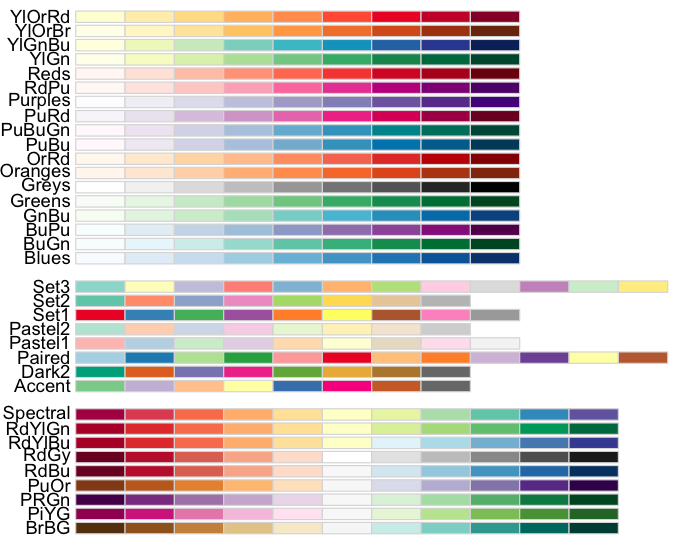
\includegraphics[scale=0.25]{images/color_palette.png}
\end{frame}

% --------------------------------------------------------------
\begin{frame}[fragile]
\frametitle{Using a color brewer palette}
\begin{knitrout}\footnotesize
\definecolor{shadecolor}{rgb}{0.969, 0.969, 0.969}\color{fgcolor}\begin{kframe}
\begin{alltt}
df  <- \hlfunctioncall{melt}(iris, id.vars = \hlstring{"Species"})
\hlfunctioncall{ggplot}(df, \hlfunctioncall{aes}(Species, value, fill = variable)) +
\hlfunctioncall{geom_bar}(stat = \hlstring{"identity"}, position = \hlstring{"dodge"}) +
\hlfunctioncall{scale_fill_brewer}(palette = \hlstring{"Set1"})
\end{alltt}
\end{kframe}
\includegraphics[width=.75\linewidth]{figure/barcolors} 

\end{knitrout}

\end{frame}

% --------------------------------------------------------------
\begin{frame}[fragile]
\frametitle{Manual color scale}
\begin{knitrout}\footnotesize
\definecolor{shadecolor}{rgb}{0.969, 0.969, 0.969}\color{fgcolor}\begin{kframe}
\begin{alltt}
\hlfunctioncall{ggplot}(iris, \hlfunctioncall{aes}(Sepal.Length, Sepal.Width, color = Species)) +
\hlfunctioncall{geom_point}() +
\hlfunctioncall{facet_grid}(Species ~ .) +
\hlfunctioncall{scale_color_manual}(values = \hlfunctioncall{c}(\hlstring{"red"}, \hlstring{"green"}, \hlstring{"blue"}))
\end{alltt}
\end{kframe}
\includegraphics[width=.75\linewidth]{figure/facetgridcolors} 

\end{knitrout}

\end{frame}

% --------------------------------------------------------------
\begin{frame}[fragile]
\frametitle{Refer to a color chart for beautful visualizations}
\url{http://tools.medialab.sciences-po.fr/iwanthue/}
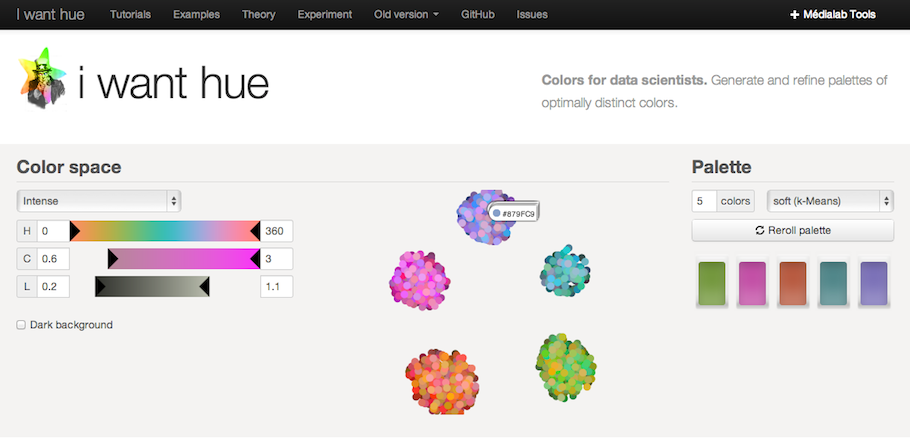
\includegraphics[scale=0.25]{images/color_schemes.png}
\end{frame}

% -----------------------------------

\section*{Faceting}
\frame{\sectionpage}

\begin{frame}[fragile]
\frametitle{Faceting along columns}
\begin{knitrout}\footnotesize
\definecolor{shadecolor}{rgb}{0.969, 0.969, 0.969}\color{fgcolor}\begin{kframe}
\begin{alltt}
\hlfunctioncall{ggplot}(iris, \hlfunctioncall{aes}(Sepal.Length, Sepal.Width, color = Species)) +
\hlfunctioncall{geom_point}() +
\hlfunctioncall{facet_grid}(Species ~ .)
\end{alltt}
\end{kframe}
\includegraphics[width=.75\linewidth]{figure/facetgrid1} 

\end{knitrout}

\end{frame}

% --------------------------------------------------------------
\begin{frame}[fragile]
\frametitle{and along rows}
\begin{knitrout}\footnotesize
\definecolor{shadecolor}{rgb}{0.969, 0.969, 0.969}\color{fgcolor}\begin{kframe}
\begin{alltt}
\hlfunctioncall{ggplot}(iris, \hlfunctioncall{aes}(Sepal.Length, Sepal.Width, color = Species)) +
\hlfunctioncall{geom_point}() +
\hlfunctioncall{facet_grid}(. ~ Species)
\end{alltt}
\end{kframe}
\includegraphics[width=.75\linewidth]{figure/facet_grid2} 

\end{knitrout}

\end{frame}

% --------------------------------------------------------------
\begin{frame}[fragile]
\frametitle{or just wrap your panels}
\begin{knitrout}\footnotesize
\definecolor{shadecolor}{rgb}{0.969, 0.969, 0.969}\color{fgcolor}\begin{kframe}
\begin{alltt}
\hlfunctioncall{ggplot}(iris, \hlfunctioncall{aes}(Sepal.Length, Sepal.Width, color = Species)) +
\hlfunctioncall{geom_point}() +
\hlfunctioncall{facet_wrap}( ~ Species)
\end{alltt}
\end{kframe}
\includegraphics[width=.75\linewidth]{figure/facet_wrap} 

\end{knitrout}

\end{frame}

% --------------------------------------------------------------
\section*{Adding smoothers}
\frame{\sectionpage}


% --------------------------------------------------------------
\begin{frame}[fragile]
\begin{knitrout}\footnotesize
\definecolor{shadecolor}{rgb}{0.969, 0.969, 0.969}\color{fgcolor}\begin{kframe}
\begin{alltt}
\hlfunctioncall{ggplot}(iris, \hlfunctioncall{aes}(Sepal.Length, Sepal.Width, color = Species)) +
\hlfunctioncall{geom_point}(\hlfunctioncall{aes}(shape = Species), size = 3) +
\hlfunctioncall{geom_smooth}(method = \hlstring{"lm"})
\end{alltt}
\end{kframe}
\includegraphics[width=.75\linewidth]{figure/adding_stats_} 

\end{knitrout}

\end{frame}

% --------------------------------------------------------------
\begin{frame}[fragile]
\begin{knitrout}\footnotesize
\definecolor{shadecolor}{rgb}{0.969, 0.969, 0.969}\color{fgcolor}\begin{kframe}
\begin{alltt}
\hlfunctioncall{ggplot}(iris, \hlfunctioncall{aes}(Sepal.Length, Sepal.Width, color = Species)) +
\hlfunctioncall{geom_point}(\hlfunctioncall{aes}(shape = Species), size = 3) +
\hlfunctioncall{geom_smooth}(method = \hlstring{"lm"}) +
\hlfunctioncall{facet_grid}(. ~ Species)
\end{alltt}
\end{kframe}
\includegraphics[width=.75\linewidth]{figure/adding_stats2_} 

\end{knitrout}

\end{frame}

% --------------------------------------------------------------
\section*{Themes}
\frame{\sectionpage}

% --------------------------------------------------------------
\begin{frame}[fragile]
\frametitle{Adding themes}
Themes are a great way to define custom plots.
\begin{knitrout}\footnotesize
\definecolor{shadecolor}{rgb}{0.969, 0.969, 0.969}\color{fgcolor}\begin{kframe}
\begin{alltt}
+\hlfunctioncall{theme}()
\hlcomment{# see ?theme() for more options}
\end{alltt}
\end{kframe}
\end{knitrout}


\end{frame}


% --------------------------------------------------------------
\begin{frame}[fragile]
\frametitle{A themed plot}
\begin{knitrout}\footnotesize
\definecolor{shadecolor}{rgb}{0.969, 0.969, 0.969}\color{fgcolor}\begin{kframe}
\begin{alltt}
\hlfunctioncall{ggplot}(iris, \hlfunctioncall{aes}(Sepal.Length, Sepal.Width, color = Species)) +
\hlfunctioncall{geom_point}(size = 1.2, shape = 16) +
\hlfunctioncall{facet_wrap}( ~ Species) +
\hlfunctioncall{theme}(legend.key = \hlfunctioncall{element_rect}(fill = NA),
legend.position = \hlstring{"bottom"},
strip.background = \hlfunctioncall{element_rect}(fill = NA),
axis.title.y = \hlfunctioncall{element_text}(angle = 0))
\end{alltt}
\end{kframe}
\end{knitrout}

\end{frame}

% --------------------------------------------------------------
\begin{frame}[fragile]
\frametitle{Adding themes}
\begin{knitrout}\footnotesize
\definecolor{shadecolor}{rgb}{0.969, 0.969, 0.969}\color{fgcolor}
\includegraphics[width=.75\linewidth]{figure/facet_wrap_theme_execc} 

\end{knitrout}

\end{frame}

% --------------------------------------------------------------
\begin{frame}[fragile]
\frametitle{ggthemes library}
\begin{knitrout}\footnotesize
\definecolor{shadecolor}{rgb}{0.969, 0.969, 0.969}\color{fgcolor}\begin{kframe}
\begin{alltt}
\hlfunctioncall{install.packages}(\hlstring{"ggthemes"})
\hlfunctioncall{library}(ggthemes)
\hlcomment{# Then add one of these themes to your plot}
+\hlfunctioncall{theme_stata}()
+\hlfunctioncall{theme_excel}()
+\hlfunctioncall{theme_wsj}()
+\hlfunctioncall{theme_solarized}()
\end{alltt}
\end{kframe}
\end{knitrout}

\end{frame}


% --------------------------------------------------------------
\section*{Create functions to automate your plotting}
\frame{\sectionpage}

% --------------------------------------------------------------
\begin{frame}[fragile]
\frametitle{Write functions for day to day plots}
\begin{knitrout}\footnotesize
\definecolor{shadecolor}{rgb}{0.969, 0.969, 0.969}\color{fgcolor}\begin{kframe}
\begin{alltt}
my_custom_plot <- \hlfunctioncall{function}(df) \{
    \hlfunctioncall{ggplot}(df, ...)
\}
\end{alltt}
\end{kframe}
\end{knitrout}

\end{frame}

% --------------------------------------------------------------
\section*{Scales}
\frame{\sectionpage}

% --------------------------------------------------------------
\begin{frame}[fragile]
\frametitle{Commonly used scales}
\begin{knitrout}\footnotesize
\definecolor{shadecolor}{rgb}{0.969, 0.969, 0.969}\color{fgcolor}\begin{kframe}
\begin{alltt}
\hlfunctioncall{scale_fill_discrete}(), \hlfunctioncall{scale_colour_discrete}()
\hlfunctioncall{scale_fill_hue}(), \hlfunctioncall{scale_color_hue}()
\hlfunctioncall{scale_fill_manual}(),  \hlfunctioncall{scale_color_manual}()
\hlfunctioncall{scale_fill_brewer}(), \hlfunctioncall{scale_color_brewer}()
\hlfunctioncall{scale_linetype}(), \hlfunctioncall{scale_shape_manual}()
\end{alltt}
\end{kframe}
\end{knitrout}

\end{frame}

% --------------------------------------------------------------
\begin{frame}[fragile]
\frametitle{Adding a continuous scale}
\begin{knitrout}\footnotesize
\definecolor{shadecolor}{rgb}{0.969, 0.969, 0.969}\color{fgcolor}\begin{kframe}
\begin{alltt}
\hlfunctioncall{library}(MASS)
\hlfunctioncall{ggplot}(birthwt, \hlfunctioncall{aes}(\hlfunctioncall{factor}(race), bwt)) +
\hlfunctioncall{geom_boxplot}(width = .2) +
\hlfunctioncall{scale_y_continuous}(labels = (\hlfunctioncall{paste0}(1:4, \hlstring{" Kg"})),
breaks = \hlfunctioncall{seq}(1000, 4000, by = 1000))
\end{alltt}
\end{kframe}
\includegraphics[width=.75\linewidth]{figure/boxplots3_} 

\end{knitrout}

\end{frame}


% --------------------------------------------------------------
\begin{frame}[fragile]
\frametitle{Another example}
\begin{knitrout}\footnotesize
\definecolor{shadecolor}{rgb}{0.969, 0.969, 0.969}\color{fgcolor}\begin{kframe}
\begin{alltt}
\hlcomment{# Assign the plot to an object}
dd <- \hlfunctioncall{ggplot}(iris, \hlfunctioncall{aes}(Sepal.Length, Sepal.Width, color = Species)) +
\hlfunctioncall{geom_point}(size = 4, shape = 16) +
\hlfunctioncall{facet_grid}(. ~Species)
\hlcomment{# Now add a scale}
dd +
\hlfunctioncall{scale_y_continuous}(breaks = \hlfunctioncall{seq}(2, 8, by = 1),
labels = \hlfunctioncall{paste0}(2:8, \hlstring{" cm"}))
\end{alltt}
\end{kframe}
\end{knitrout}

\end{frame}



% --------------------------------------------------------------
\section*{Publication quality figures}
\frame{\sectionpage}

% How to save your plots
% --------------------------------------------------------------
\begin{frame}[fragile]
\begin{itemize}
\item If the plot is on your screen
\begin{knitrout}\footnotesize
\definecolor{shadecolor}{rgb}{0.969, 0.969, 0.969}\color{fgcolor}\begin{kframe}
\begin{alltt}
\hlfunctioncall{ggsave}(\hlstring{"~/path/to/figure/filename.png"})
\end{alltt}
\end{kframe}
\end{knitrout}

\item If your plot is assigned to an object
\begin{knitrout}\footnotesize
\definecolor{shadecolor}{rgb}{0.969, 0.969, 0.969}\color{fgcolor}\begin{kframe}
\begin{alltt}
\hlfunctioncall{ggsave}(plot1, file = \hlstring{"~/path/to/figure/filename.png"})
\end{alltt}
\end{kframe}
\end{knitrout}


\item Specify a size
\begin{knitrout}\footnotesize
\definecolor{shadecolor}{rgb}{0.969, 0.969, 0.969}\color{fgcolor}\begin{kframe}
\begin{alltt}
\hlfunctioncall{ggsave}(file = \hlstring{"/path/to/figure/filename.png"}, width = 6,
height =4)
\end{alltt}
\end{kframe}
\end{knitrout}

\item or any format (pdf, png, eps, svg, jpg)
\begin{knitrout}\footnotesize
\definecolor{shadecolor}{rgb}{0.969, 0.969, 0.969}\color{fgcolor}\begin{kframe}
\begin{alltt}
\hlfunctioncall{ggsave}(file = \hlstring{"/path/to/figure/filename.eps"})
\hlfunctioncall{ggsave}(file = \hlstring{"/path/to/figure/filename.jpg"})
\hlfunctioncall{ggsave}(file = \hlstring{"/path/to/figure/filename.pdf"})
\end{alltt}
\end{kframe}
\end{knitrout}

\end{itemize}
\end{frame}

% --------------------------------------------------------------
\begin{frame}[fragile]
\frametitle{Further help}
\begin{itemize}
\item You've just scratched the surface with ggplot2.
\item Practice
\item Read the docs (either locally in \texttt{R} or at \url{http://docs.ggplot2.org/current/})
\item Work together
\end{itemize}

\includegraphics[scale=.15]{images/chang_book.png}
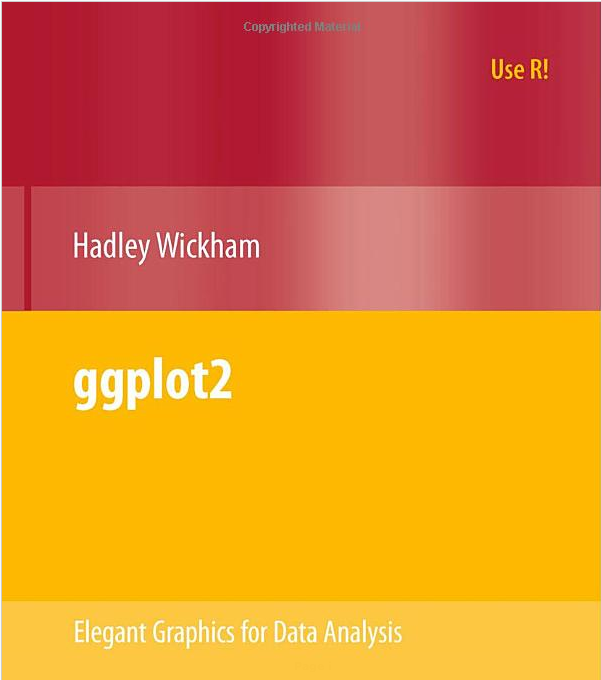
\includegraphics[scale=.15]{images/hadley.png}
\end{frame}

% --------------------------------------------------------------
% end, hope it was useful.
\end{document}
